%TODO: hässlichen newpage entfernen
\newpage

\section{Gebräuchliche Realisierung von OTA's}
Ein einstufiger OTA wird bereits durch die Differenzstufe realisiert. Dies ist jedoch nicht praktisch da die Last am
Ausgang die Symmetrie der Differenzstufe stört.
Schaltungen siehe Abbildung \ref{fig:otas}!
\begin{figure}[htp]
\begin{center}
	\begin{subfigure}[b]{0.49\linewidth}
		\centering
		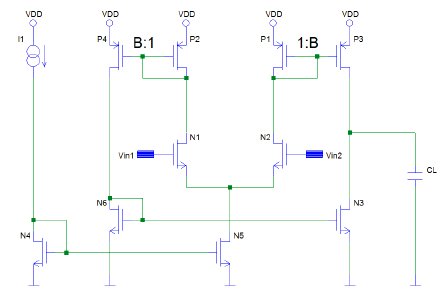
\includegraphics[width=0.9\linewidth]{images/SymetrischerOTA.png}
		\caption{Symmetrischer OTA}
	\end{subfigure}
	\begin{subfigure}[b]{0.49\linewidth}
		\centering
		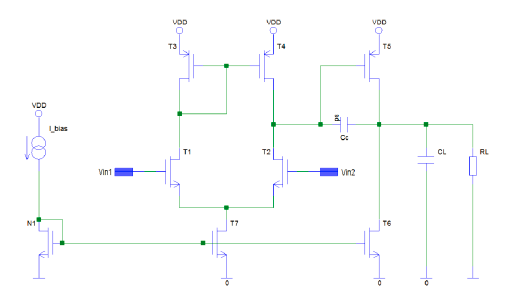
\includegraphics[width=0.9\linewidth]{images/millerOTA.png}
		\caption{Miller OTA}
	\end{subfigure}
	\caption{Gebräuchliche Realisierungen von OTA's}
	\label{fig:otas}
\end{center}
\end{figure}

\textbf{Verstärkungen:} \\
\begin{tabular}{lll}
	Symmetrischer OTA:	& & $a_v = B \cdot g_{m_{N1}} \cdot (r_{DS_{N3}} || r_{DS_{P3}})$ \\
	Miller OTA:			& & $a_v = a_{v1} \cdot a_{v2} = g_{m1}(r_{DS2} || r_{DS4}) \cdot g_{m5}(r_{DS5} || r_{DS6} || R_L)$
\end{tabular}

\subsection{Designgleichungen Miller OTA}
\begin{tabular}{|l|l|} \hline
	Verstärkung & $a = A_1 \cdot A_2 = g_{m1} \cdot R_{N2} \cdot g_{m5} \cdot R_{N3}$ \\ \hline
	Dominanter Pol & $f_{pN2} = \frac{1}{2\pi R_{N2} (C_{N2}+A_2C_c)} \approx \frac{1}{2\pi R_{N2}A_2C_c}$ \\ \hline
	3dB-Bandwidth & $BW \approx f_d = f_{N2} = \frac{1}{2\pi \cdot R_{N2} \cdot A_2C_c}$ \\ \hline
	Gain-Bandwith & $GBP = a \cdot f_d = \frac{g_{m1} \cdot R_{N2} \cdot g_{m5} \cdot R_{N3}}{2\pi \cdot R_{N2} \cdot A_2C_c} = \frac{g_{m1}}{2\pi C_c}$ \\ \hline
	Nondominanter Pol & $f_{nd} = f_{N3} = \frac{1}{2\pi \cdot R_{N3} \cdot C_L} \approx \frac{g_{m5}}{2\pi C_L}$ \\ \hline
	Phasenmarge & $\phi_m = 90^\circ - \arctan \frac{GBW}{f_{nd}}$ \\ \hline
	Nullstelle & $f_z \approx \frac{g_{m5}}{2\pi C_c}$ \\ \hline
\end{tabular}